\documentclass{article}
\usepackage{graphicx}
\usepackage{amsmath,amsthm,amssymb}
\usepackage[font=small,labelfont=bf]{caption}
\usepackage{tikz}
\usepackage{pgfplots}
\pgfplotsset{compat=1.18}
\usetikzlibrary{calc, angles, quotes, shapes.geometric, decorations.pathreplacing}
\usepackage{tkz-euclide}
\usepackage[inline]{asymptote}
\usepackage{float}
\usepackage[margin=1in]{geometry}
\usepackage{gensymb}
\usepackage[normalem]{ulem}
\usepackage{hyperref}
\hypersetup{
    colorlinks=true,
    linkcolor=blue,
    filecolor=magenta,      
    urlcolor=cyan,
    pdftitle={Overleaf Example},
    pdfpagemode=FullScreen,
    }
\usepackage{fancyhdr}
\pagestyle{fancy}
\fancyhead[R]{Enoch Yu}
\pagenumbering{gobble}
\usepackage{enumitem}
\newtheorem{theorem}{Theorem}[section]
\newtheorem{lemma}[theorem]{Lemma}
\newtheorem*{lemma*}{Lemma}
\newtheorem{sublemma}{Lemma}[section]
\newtheorem{proposition}{Proposition}
\newtheorem{corollary}{Corollary}[theorem]
\newtheorem{example}{Example}[section]
\newtheorem*{example*}{Example}
\newtheorem{hypothesis}{Hypothesis}[section]
\newtheorem*{hypothesis*}{Hypothesis}
\newenvironment{solution}{\begin{trivlist}\item[]{\bf Solution}}{\qed \end{trivlist}}
\newcommand{\verteq}{\rotatebox{90}{$\;\;=\;\;$}}
\newcommand*\circled[1]{\tikz[baseline=(char.base)]{
            \node[shape=circle,draw,inner sep=1pt] (char) {#1};}}
\newcommand{\triangled}[1]{\tikz[baseline=(char.base)]{
            \node[shape=regular polygon, regular polygon sides=3, draw, inner sep=0.2pt] (char) {#1};}}

\title{Problem Set 25}
\author{Enoch Yu}
\date{June 2025}

\begin{document}

\section*{Problem}
Show that in $\triangle{ABC}$, we have $4\cos\frac{A}{2}\cos\frac{B}{2}\cos\frac{C}{2}=\frac{s}{R}$.
\\\\
\textbf{Possible Trigger}
\begin{center}
    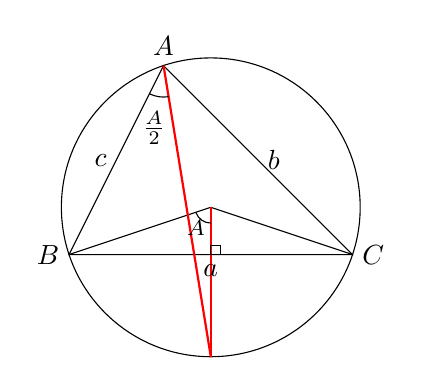
\begin{tikzpicture}[scale=0.6]
        \coordinate (A) at (2,4);
        \coordinate (B) at (0,0);
        \coordinate (C) at (6,0);
        \coordinate (O) at (3,1);
        \coordinate (D) at (3,-2.16);
        \coordinate (E) at (3, 0);

        \draw (A) -- (B) -- (C) -- cycle;
        \draw (O) circle (3.16227766017);

        \draw (O) -- (B);
        \draw (O) -- (C);

        \draw[red, thick] (O) -- (D);
        \draw[red, thick] (A) -- (D);

        \draw pic["\footnotesize $A$", draw=black, angle radius=0.2cm, angle eccentricity=1.6] {angle=B--O--D};
        \draw pic["$\frac{A}{2}$", draw=black, angle radius=0.4cm, angle eccentricity=2] {angle=B--A--D};

        \tkzMarkRightAngle[size=.2](O,E,C);

        \node[above] at (A) {$A$};
        \node[left] at (B) {$B$};
        \node[right] at (C) {$C$};

        \node[left] at ($(A)!0.5!(B)$) {$c$};
        \node[right] at ($(A)!0.5!(C)$) {$b$};
        \node[below] at ($(C)!0.5!(B)$) {$a$};
    \end{tikzpicture}
\end{center}
Unfortunately, the trigger cannot be utilize since not much of the lengths are known.
\begin{proof}
Half Angle Formula and the Law of Cosines could be utilized.
\begin{align*}
    \cos A &= \frac{b^2 + c^2 - a^2}{2bc} \\[0.5em]
    \cos\frac{A}{2}
    &= \sqrt{\frac{1 + \frac{b^2 + c^2 - a^2}{2bc}}{2}} = \sqrt{\frac{b^2 + 2bc + c^2 - a^2}{4bc}} \\[0.5em]
    &= \sqrt{\frac{(b + c)^2 - a^2}{4bc}} = \sqrt{\frac{(a + b + c)(-a + b + c)}{4bc}} \\[0.5em]
    &= \sqrt{\frac{s(s - a)}{bc}}
\end{align*}
The form triggers area formulas such as Heron's Formula and area using the radius of circumcircle.
\begin{align*}
    4 \cdot \sqrt{\frac{s(s - a)}{bc}} \cdot \sqrt{\frac{s(s - b)}{ac}} \cdot \sqrt{\frac{s(s - c)}{ab}}
    &= 4 \cdot \sqrt{\frac{s^3(s - a)(s - b)(s - c)}{a^2b^2c^2}} \\[0.5em]
    &= \frac{4s}{abc} \cdot \sqrt{s(s - a)(s - b)(s - c)} = \frac{4s}{abc} \cdot \frac{abc}{4R} \\[0.5em]
    &= \frac{s}{R}
\end{align*}
\end{proof}

\section*{Problem}
In $\triangle{ABC}$, the angles $A$, $B$, and $C$ satisfy the equation $\cos A \cos B + \sin A \sin B \sin C = 1$. Determine all possible values of $\angle{C}$.
\begin{solution}
$\cos A \cos B + \sin A \sin B$ reminds me of $\cos(A - B)$.
\begin{align*}
    \cos(A - B) - \sin A \sin B + \sin A \sin B \sin C &= 1 \\
    \cos(A - B) &= 1 + \sin A \sin B (1 - \sin C)
\end{align*}
Notice that the left hand side is in the interval $[-1, 1]$. In other words, because $\sin A$ and $\sin B$ are always positive, $\sin C = 1$. The only possible case is when $\boxed{m\angle{C} = 90^\circ}$.
\end{solution}

\newpage
\section*{Problem}
Let $\triangle{ABC}$ be an acute triangle whose altitudes meet at point $H$, and let $X$ be on $\overline{BC}$ such that $\overline{AX} \perp \overline{BC}$. Show that $HX = 2R \cos B \cos C$.
\begin{proof}
First and foremost, WLOG, the diagram could be drawn.
\begin{center}
    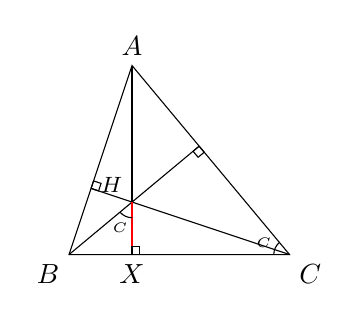
\begin{tikzpicture}[scale=0.4]
        \coordinate (A) at (2,6);
        \coordinate (B) at (0,0);
        \coordinate (C) at (7,0);
        \coordinate (X) at (2,0);
        \coordinate (Y) at (4.13,3.44);
        \coordinate (Z) at (0.7,2.1);
        \coordinate (H) at (2,1.67);

        \draw (A) -- (B) -- (C) -- cycle;
        \draw (A) -- (X);
        \draw (B) -- (Y);
        \draw (C) -- (Z);

        \draw[red, thick] (H) -- (X);
 
        \draw pic["\tiny $C$", draw=black, angle radius=0.2cm, angle eccentricity=1.8] {angle=A--C--X};
        \draw pic["\tiny $C$", draw=black, angle radius=0.2cm, angle eccentricity=1.8] {angle=B--H--X};

        \tkzMarkRightAngle[size=.25](C,Z,A);
        \tkzMarkRightAngle[size=.25](B,Y,C);
        \tkzMarkRightAngle[size=.25](A,X,C);

        \node[above] at (A) {$A$};
        \node[above left] at (H) {\footnotesize $H$};
        \node[below left] at (B) {$B$};
        \node[below] at (X) {$X$};
        \node[below right] at (C) {$C$};
    \end{tikzpicture}
\end{center}
Using trigonometric identities and law of sines, the following equations could be proven.
\begin{align*}
    HX = BX \cdot \frac{1}{\tan C}
    &= BX \cdot \cot C \\
    &= AB \cdot \cos B \cdot \frac{\cos C}{\sin C} \\
    &= \frac{AB}{\sin C} \cdot \cos B \cos C \\
    &= 2R \cos B \cos C
\end{align*}
\end{proof}

\section*{Problem}
In triangle $ABC$, $D$ is on $\overline{AC}$ and $F$ is on $\overline{BC}$. Also, $\overline{AB} \perp \overline{AC}$, $\overline{AF} \perp \overline{BC}$, and $BD = DC = FC = 1$. Find $\overline{AC}$.
\begin{solution}
\\\\
Similar triangle could be used to solve the problem. However, because methods with similar triangles are way too common, let's try something new like using trigonometric identities.
\begin{center}
    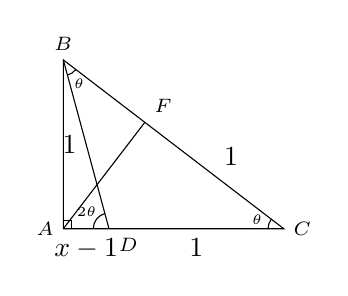
\begin{tikzpicture}[scale=0.4]
        \coordinate (A) at (0,0);
        \coordinate (B) at (0,5.36);
        \coordinate (C) at (7,0);
        \coordinate (D) at (1.45,0);
        \coordinate (F) at (2.59,3.38);
    
        \draw (A) -- (B) -- (C) -- cycle;
    
        \draw (A) -- (F);
        \draw (B) -- (D);

        \draw pic["\tiny $\theta$", draw=black, angle radius=0.2cm, angle eccentricity=1.8] {angle=D--B--C};
        \draw pic["\tiny $\theta$", draw=black, angle radius=0.2cm, angle eccentricity=1.8] {angle=F--C--D};
        \draw pic["\tiny $2\theta$", draw=black, angle radius=0.2cm, angle eccentricity=1.8] {angle=B--D--A};

        \tkzMarkRightAngle[size=.25](B,A,C);

        \node[below] at ($(D)!0.5!(C)$) {$1$};
        \node[above right] at ($(F)!0.5!(C)$) {$1$};
        \node[left] at ($(D)!0.5!(B)$) {$1$};

        \node[below] at ($(D)!0.5!(A)$) {$x-1$};

        \node[left] at (A) {\scriptsize $A$};
        \node[above] at (B) {\scriptsize $B$};
        \node[right] at (C) {\scriptsize $C$};
        \node[below right] at (D) {\scriptsize $D$};
        \node[above right] at (F) {\scriptsize $F$};
    \end{tikzpicture}
\end{center}
Trigonometric identities could be utilized.
\begin{align*}
    \cos2\theta &= 2\cos^2\theta - 1 \\
    \frac{x - 1}{1} &= 2 \cdot \left( \frac{1}{x} \right)^2 - 1 \\
    x^3 - x^2 &= 2 - x^2 \\
    \therefore x &= \boxed{\sqrt[3]{2}} \quad (\because x \in \mathbb{R})
\end{align*}
\end{solution}

\newpage
\section*{2005 AIME I Problem 7}
In quadrilateral $ABCD$, $BC = 8$, $CD = 12$, $AD = 10$, and $\angle{A} = \angle{B} = 60^{\circ}$. Find $AB$.
\begin{solution}
\begin{center}
    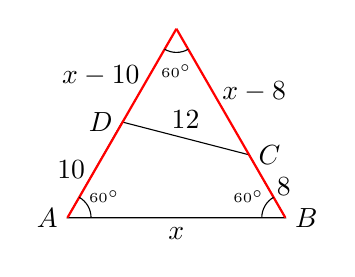
\begin{tikzpicture}[scale=0.8]
        \coordinate (A) at (0,0);
        \coordinate (B) at (3.46,0);
        \coordinate (C) at (2.88,1);
        \coordinate (D) at (0.87,1.52);
        \coordinate (E) at (1.73,3);

        \draw (A) -- (B) -- (C) -- (D) -- cycle;
        \draw[thick, red] (E) -- (A);
        \draw[thick, red] (E) -- (B);

        \node[left] at ($(D)!0.5!(A)$) {$10$};
        \node[below] at ($(B)!0.5!(A)$) {$x$};
        \node[right] at ($(B)!0.5!(C)$) {$8$};
        \node[above] at ($(D)!0.5!(C)$) {$12$};
        \node[left] at ($(E)!0.5!(D)$) {$x-10$};
        \node[right] at ($(E)!0.5!(C)$) {$x-8$};

        \draw pic["\tiny $60^\circ$", draw=black, angle radius=0.3cm, angle eccentricity=1.8] {angle=D--E--C};
        \draw pic["\tiny $60^\circ$", draw=black, angle radius=0.3cm, angle eccentricity=1.8] {angle=C--B--A};
        \draw pic["\tiny $60^\circ$", draw=black, angle radius=0.3cm, angle eccentricity=1.8] {angle=B--A--D};

        \node[left] at (A) {$A$};kaka
        
        \node[right] at (B) {$B$};
        \node[right] at (C) {$C$};
        \node[left] at (D) {$D$};
    \end{tikzpicture}
\end{center}
The law of cosines could be used.
\begin{align*}
    \cos60^\circ &= \frac{(x - 10)^2 + (x - 8)^2 - 12^2}{2(x - 10)(x - 8)} \\
    (x - 10)(x - 8) &= (x - 10)^2 + (x - 8)^2 - 12^2 \\
    \therefore x&= \boxed{9 + \sqrt{141}}
\end{align*}
\end{solution}

\section*{2004 AIME II Problem 11}
A right circular cone has a base with radius $600$ and height $200\sqrt{7}$. An ant starts at a point on the surface of the cone whose distance from the vertex of the cone is $125$, and crawls along the surface of the cone to a point on the exact opposite side of the cone whose distance from the vertex is $375\sqrt{2}$. Find the least distance that the ant could have crawled.
\begin{solution}
\begin{center}
    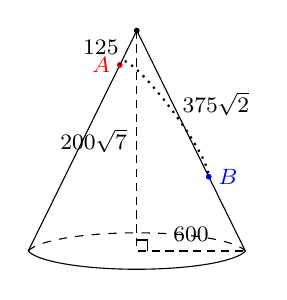
\begin{tikzpicture}[scale=0.7]
    \draw[dashed] (0,0) arc (170:10:2cm and 0.4cm)coordinate[pos=0] (a);
    \draw (0,0) arc (-170:-10:2cm and 0.4cm)coordinate (b);
    
    \draw[densely dashed] ([yshift=4cm]$(a)!0.5!(b)$) -- node[left,font=\footnotesize] {$200\sqrt{7}$}coordinate[pos=0.95] (aa)($(a)!0.5!(b)$)
                            -- node[above,font=\footnotesize] {$600$}coordinate[pos=0.1] (bb) (b);
    \draw (aa) -| (bb);

    \draw (a) -- ([yshift=4cm]$(a)!0.5!(b)$) -- (b);

    \coordinate (V) at ([yshift=4cm]$(a)!0.5!(b)$);

    \path (V) -- (a) coordinate[pos=0.15625] (A);
    \fill[red] (A) circle (1.5pt) node[left] {\footnotesize $A$};

    \pgfmathsetmacro{\Bfrac}{375*sqrt(2)/800}
    \path (V) -- (b) coordinate[pos=\Bfrac] (B);
    \fill[blue] (B) circle (1.5pt) node[right] {\footnotesize $B$};

    \fill (V) circle (1.5pt);

    \node[left] at ($(A)!0.5!(V)$) {\footnotesize $125$};
    \node[right] at ($(B)!0.5!(V)$) {\footnotesize $375\sqrt{2}$};

    \draw[thick, dotted] 
        (A) .. controls ++(0,0.5) and ++(0,0.5) .. (B);
\end{tikzpicture}
\end{center}

\noindent
To find the shortest length from the red to blue points, the net of the side of the cone could be drawn.

\begin{center}
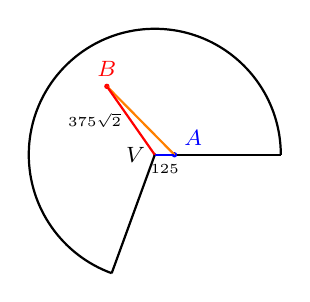
\begin{tikzpicture}[scale=0.02]
    \def\R{80}
    \def\theta{250}
    \def\A{12.5}
    \def\B{53.033}

    \draw[thick] (0,0) -- (\theta:\R);
    \draw[thick] (0,0) -- (0:\R);
    \draw[thick] (0:\R) arc (0:\theta:\R);

    \fill (0,0) circle (1.2);

    \coordinate (o) at (0,0) node[left] {\footnotesize $V$};

    \coordinate (a) at (0:\A);
    \fill[blue] (a) circle (1.7) node[above right] {\footnotesize $A$};

    \coordinate (b) at ({\theta/2}:\B);
    \fill[red] (b) circle (1.7) node[above] {\footnotesize $B$};

    \draw[thick, orange] (a) -- (b);

    \draw[thick, blue] (o) -- (a);
    \draw[thick, red] (o) -- (b);

    \node[below] at ($(o)!0.5!(a)$) {\tiny $125$};
    \node[left] at ($(o)!0.5!(b)$) {\tiny $375\sqrt{2}$};
\end{tikzpicture}
\end{center}

\noindent
The angle $YVX$ is equal to $360^\circ \cdot \frac{1200\pi}{1600\pi} \cdot \frac{1}{2}$, or $135^\circ$. Therefore, the law of cosines could be utilized.
\[
AB = \sqrt{(375\sqrt{2})^2 + 125^2 - 2 \cdot (375\sqrt{2})(125)(\cos 135^\circ)} = \boxed{625}
\]
\end{solution}
Uploaded a \href{https://artofproblemsolving.com/wiki/index.php/2004_AIME_II_Problems/Problem_11#Solution_2}{new solution} in AOPS!! \\
\includegraphics[scale=0.05]{Screenshot 2025-06-25 at 5.54.31 PM.png}

\end{document}
